\chapter{Fundamentals} % Main chapter title

\label{Chapter2} % For referencing the chapter elsewhere, use \ref{Chapter2}
% TODO Sectionnamen: Die Namen der Sections sind nicht unbedingt sinnvoll und sind jetzt erstmal dazu da 
% mir selbst den Roten Faden aufzuzeigen
% \section{Virtual Memory}
% Grundlagen auffrischen, kurz die Motivation und Grundkonzepte von Virtual Memory erläutern
% Da eventuell kurz auf Atlas eingehen und wie sehr sich VM bis jetzt entwickelt hat
% Quellen:
% - Lehrbücher: VM Definitionen und Übersichtsbeschreibungen
% \subsection{What is Virtual Memory}


% Purpose of Section:
% Ziegen, dass es keinen Standard gibt und es viele Verschiedne Möglichkeiten gibt um VM zu realisieren
% Quellen:
% [ A look at several...]
% [ Issues of implementation]
% \section{Implementation of Virtual Memory Systems}
% \subsection{ Overview of different implementations (Inverted/Hierarchical/Multi-Level)}
% \subsection{ Comparison of differnt implementations with regards to performance and features like page sharing}

% \section{Hardware support}
% \subsection{MMU & TLB}
% \subsection{HW-Dependent PTE Structure}
% \subsection{A typical Page Table Walk}

% \section{ Sofware Paging approaches}
% \subsection{More flexibilty}

\begin{figure*}[t]
    \centering
    \begin{bytefield}[bitwidth=\widefigurewidth/39,bitheight=\widthof{~PBMT~}, bitformatting={\tiny\bfseries}, boxformatting={\centering}]{39}
        \bitheader[endianness=big]{38,30,29,21,20,12,11,0} \\
        \bitbox{9}{VPN[2]} &
        \bitbox{9}{VPN[1]} &
        \bitbox{9}{VPN[0]} &
        \bitbox{12}{Page Offset}\\
    \end{bytefield}
    \caption[RISC-V Sv39 Virtual Address]{RISC-V Sv39 Virtual Address}
    \label{fig:fundamentals:sv39va}
\end{figure*}

\begin{figure*}[t]
    \centering
    \begin{bytefield}[bitwidth=\widefigurewidth/56,bitheight=\widthof{~PBMT~}, bitformatting={\tiny\bfseries}, boxformatting={\centering}]{56}
        \bitheader[endianness=big]{55,30,29,21,20,12,11,0} \\
        \bitbox{26}{PPN[2]} &
        \bitbox{9}{PPN[1]} &
        \bitbox{9}{PPN[0]} &
        \bitbox{12}{Page Offset}\\
    \end{bytefield}
    \caption[RISC-V Sv39 Physical Address]{RISC-V Sv39 Physical Address}
    \label{fig:fundamentals:sv39pa}
\end{figure*}

\begin{figure*}[t]
    \centering
    \begin{bytefield}[bitwidth=\widefigurewidth/64,bitheight=\widthof{~PBMT~}, bitformatting={\tiny\bfseries}, boxformatting={\centering}]{64}
        \bitheader[endianness=big]{63,62,61,60,54,53,28,27,19,18,10,9,8,7,6,5,4,3,2,1,0} \\
        \bitbox{1}{N} &
        \bitbox{2}{\rotatebox{90}{PBMT}} &
        \bitbox{7}{Reserved} &
        \bitbox{26}{PPN[2]} &
        \bitbox{9}{PPN[1]} &
        \bitbox{9}{PPN[0]} &
        \bitbox{2}{\rotatebox{90}{RSW}} &
        \bitbox{1}{D} &
        \bitbox{1}{A} &
        \bitbox{1}{G} &
        \bitbox{1}{U} &
        \bitbox{1}{X} &
        \bitbox{1}{W} &
        \bitbox{1}{R} &
        \bitbox{1}{V}
    \end{bytefield}
    \caption[RISC-V Sv39 Page Table Entry]{RISC-V Sv39 Page Table Entry}
    \label{fig:fundamentals:sv39pte}
\end{figure*}
\
\begin{figure*}[ht]
    \centering
    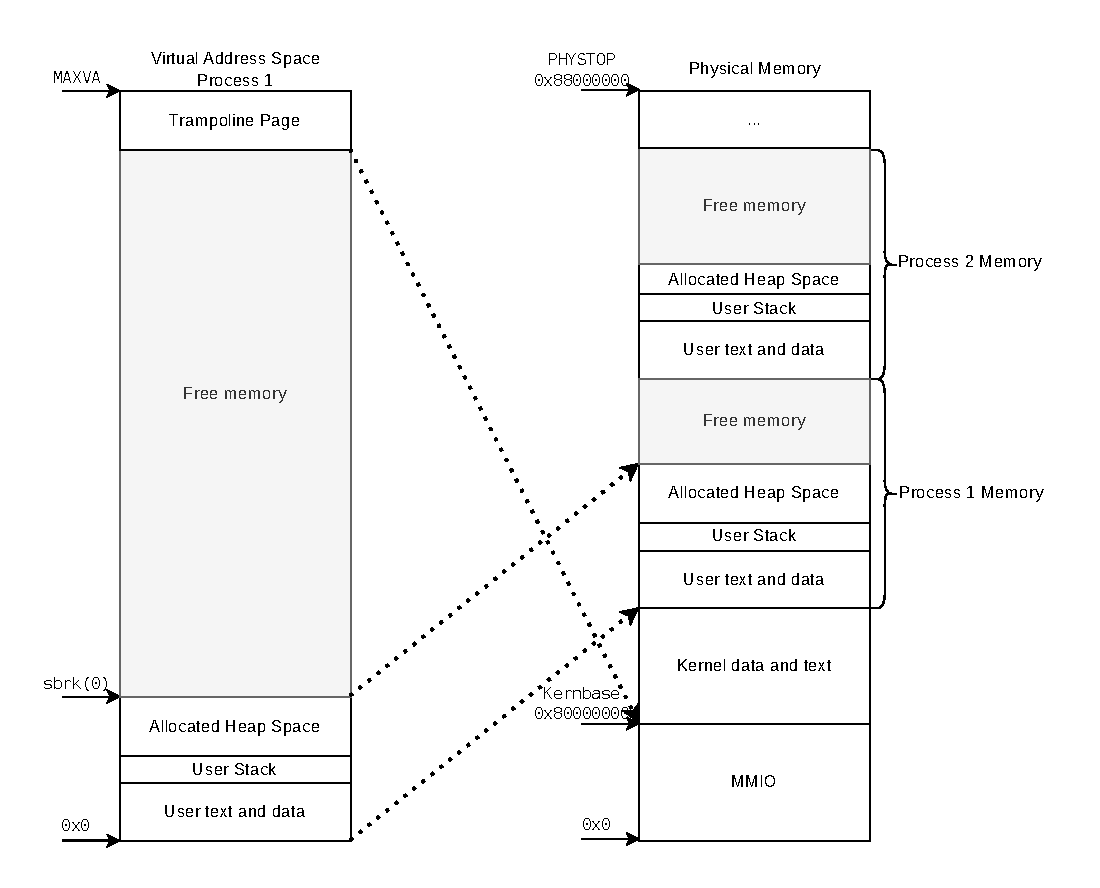
\includegraphics[]{figures/simple_mapping.pdf}

    \caption[Simple Mapping Scheme]{Simple Mapping Scheme}
    \label{fig:theory:simplemapping}
\end{figure*}